\chapter{Aufgabenstellung} \label{ch:Aufgabe}
Modelliert werden sollen die Reaktionsgleichung
\begin{align}
	A_1 \ce{<=>} A_2  \ce{->} A_3
\end{align}
\begin{figure}[ht]
	\centering
	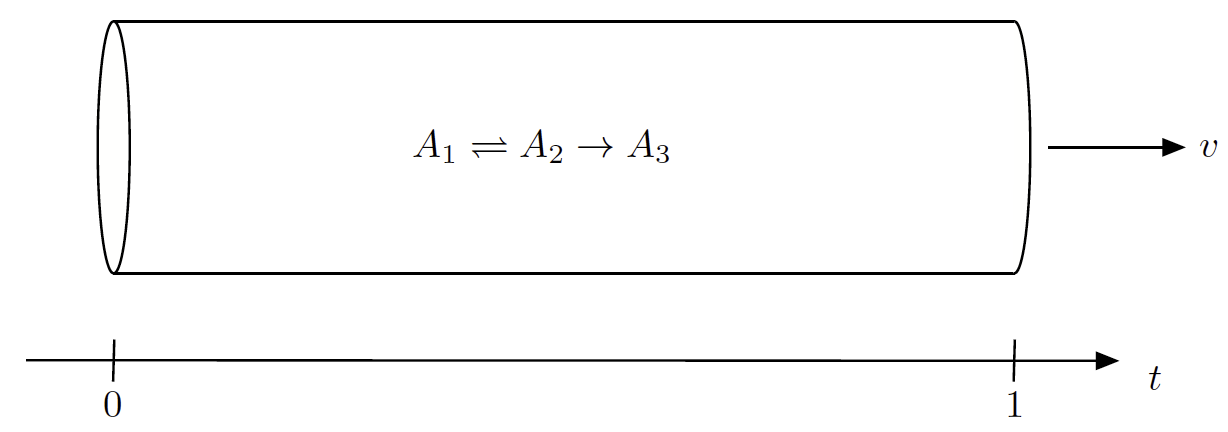
\includegraphics[width=1\textwidth]{images/PlugFlowTubeReactor.png}
	\caption{\label{fig:PFTR}Plug Flow Tube Reactor}
\end{figure}

Dabei seien
\begin{itemize}
	\item $x_1(t)$: Konzentration von $A_1$
	\item $x_2(t)$: Konzentration von $A_2$
	\item $\vartheta(t)$: ortsabhängige Temperatur im Reaktor
	\item $u(t)$: transformierte Steuerung.
\end{itemize}

Die Dynamik des Systems lässt sich durch
\begin{align}
	&\dot{x}_1(t) = -k_1x_1(t)+k_2x_2(t)\\
	&\dot{x}_2(t)= k_1x_1(t)-(k_2+k_3)x_2(t)
\end{align}
beschreiben, wobei die Reaktionsraten $k_1$, $k_2$ und $k_3$ von der ortsabhängigen Temperatur im Reaktor abhängen. Hierfür gilt
\begin{align}
	&k_1 = \exp\left(-\frac{\alpha}{\vartheta(t)}\right), \alpha > 0 \label{eq:k1} \\ 
	&k_2 = k_1^2\\
	&k_3 = 2k_1^2
\end{align}
und $\vartheta_{min} \leq \vartheta(t) \leq \vartheta_{max}$. Das Ziel ist die Temperatur so zu steuern, dass die Produktausbeute von $A_2$ am
Ende des Vorgangs maximal wird. Mit der transformierten Steuervariable $u(t) = k_1(t) = \exp\left(-\alpha/\vartheta(t)\right)$ ergibt sich folgendes Optimalsteuerungsproblem
\begin{align}
	&\min_u -x_2(1)\\\nonumber
	&\st &&Dynamik:\\\nonumber
	&&&\dot{x}_1(t) = -ux_1(t)+u^2x_2(t)\\\nonumber
	&&&\dot{x}_2(t) = ux_1(t) - 3u^2x_2(t)\\\nonumber
	&&&Anfangs-/ Steuerbedingungen:\\\nonumber
	&&&x_1(0) = x_{1,0}\\\nonumber
	&&&x_2(0) = x_{2,0}\\\nonumber
	&&&u(t) \in \left[u_{min}, u_{max}\right] \: \forall t \in \left[0,1\right].\nonumber
\end{align}
Wir wählen $x_{1,0} = 1, \: x_{2,0} = 0, \:  u_{min} = 0$ und $u_{max} = 5$.